\documentclass[11pt,a4paper,bibtotoc,idxtotoc,BCOR15mm,DIV10]{scrbook}
\usepackage[utf8]{inputenc}
%\usepackage[T1]{fontenc}
%\usepackage{listings}
%\usepackage{amsmath}
%\usepackage{amsfonts}
\usepackage{graphicx}
\usepackage{tumlogo}
\usepackage{isabelle,isabellesym}

\usepackage{ifthen}
\newcommand{\clearemptydoublepage}{
  \ifthenelse{\boolean{@twoside}}{\newpage{\pagestyle{empty}\cleardoublepage}}
  {\clearpage}}
\renewcommand{\bf}{\normalfont \bfseries}
% set title, authors and stuff for the cover
\def\doctype{Bachelor's Thesis in Informatics}
\def\title{Multiple Precision Floating Point Arithmetic in Isabelle/HOL}
\def\titleEng{Multiple Precision Floating Point Arithmetic in Isabelle/HOL}
\def\author{Fabian Hellauer}
\def\date{March 15, 2016}


% further packages required for unusual symbols (see also
% isabellesym.sty), use only when needed

%\usepackage{amssymb}
  %for \<leadsto>, \<box>, \<diamond>, \<sqsupset>, \<mho>, \<Join>,
  %\<lhd>, \<lesssim>, \<greatersim>, \<lessapprox>, \<greaterapprox>,
  %\<triangleq>, \<yen>, \<lozenge>

%\usepackage{eurosym}
  %for \<euro>

%\usepackage[only,bigsqcap]{stmaryrd}
  %for \<Sqinter>

%\usepackage{eufrak}
  %for \<AA> ... \<ZZ>, \<aa> ... \<zz> (also included in amssymb)

%\usepackage{textcomp}
  %for \<onequarter>, \<onehalf>, \<threequarters>, \<degree>, \<cent>,
  %\<currency>

% this should be the last package used
\usepackage{pdfsetup}

% urls in roman style, theory text in math-similar italics
\urlstyle{rm}
\isabellestyle{it}

% for uniform font size
%\renewcommand{\isastyle}{\isastyleminor}


\begin{document}

\frontmatter

\def\hoffsettemp{\hoffset}
\setlength{\hoffset}{0pt}

\thispagestyle{empty}

\vspace{4cm}
\begin{center}

  \oTUM{4cm}

  \vspace{5mm}     
  \huge DEPARTMENT OF INFORMATICS\\ 
  \vspace{0.5cm}
  \large TECHNISCHE UNIVERSIT{\"A}T M{\"U}NCHEN\\
  \vspace{1mm}
  
\end{center}


\vspace{15mm}


\begin{center}

  {\Large \doctype}\\
  \vspace{20mm}
  {\huge\bf \title}\\%[3ex]
  \vspace{15mm}

  {\LARGE  \author}

  \vspace{10mm}

  \begin{figure}[h!]
    \centering
    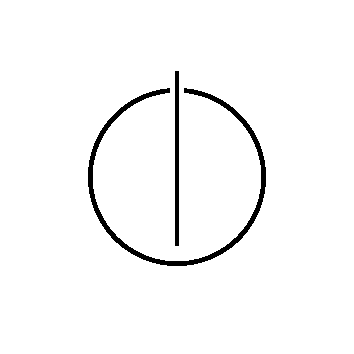
\includegraphics[width=4cm]{informat}
  \end{figure}

\end{center}

\setlength{\hoffset}{\hoffsettemp}

%%% Local Variables: 
%%% mode: latex
%%% TeX-master: "ausarbeitung"
%%% End: 


\clearemptydoublepage
\thispagestyle{empty}

 \vspace{10mm}
\begin{center}
	       \oTUM{4cm}
	   
	   \vspace{5mm}     
	   \huge DEPARTMENT OF INFORMATICS\\ 
	   \vspace{0.5cm}
	 \large TECHNISCHE UNIVERSIT{\"A}T M{\"U}NCHEN\\
        
	\end{center}
		

\vspace{10mm}
\begin{center}

   {\Large \doctype}

  \vspace{10mm}
  
  {\LARGE \title}\\
  
  
  \vspace{10mm}
  
  {\LARGE \titleEng}\\
  
  
  \vspace{10mm}

    %\hfill
    \begin{tabular}{ll}
	   \Large Author: & \Large \author \\[2mm]
	   \Large Supervisor: & \Large Prof. Tobias Nipkow \\[2mm]
	   \Large Advisor: & \Large Fabian Immler \\[2mm]				
	   \Large Submission date: & \Large \date
	 \end{tabular}
	 
	 \vspace{5mm}
	 
	 \begin{figure}[h!]
  \centering
   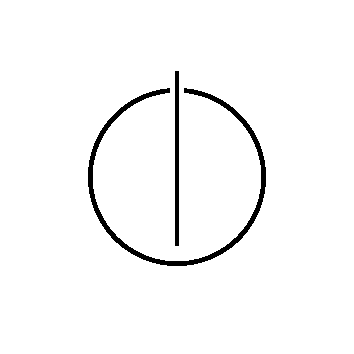
\includegraphics[width=4cm]{informat}
  \end{figure}
   

\end{center}

\clearemptydoublepage

\thispagestyle{empty} \vspace*{0.8\textheight} \noindent I confirm that this bachelor's thesis is my own work and I have documented all sources and material used.
	
	\vspace{15mm}
	\noindent
	München, \date \hspace{5cm} \author
\newpage

%%% Local Variables: 
%%% mode: plain-tex
%%% TeX-master: "ausarbeitung"
%%% End: 


\clearemptydoublepage
\addcontentsline{toc}{chapter}{Abstract}

\vspace*{2cm}
\begin{center}
{\Large \bf Abstract}
\end{center}
\vspace{1cm}
Many problems, e.g. in geometry or topology systems, need large computations with long sequences of arithmetic operations to be solved. Machine computation using hardware floating point instructions, like the one specified by the "Institute of Electrical and Electronics Engineers" (IEEE) 754 standard\cite{IEEE},  can offer a huge speedup. However, using the IEEE-floats directly would often create the need for a complicated numerical analysis due to them being affected by round-off.
However, this downside can be removed at the cost of a few extra instructions: Alongside the result, the round-off error of an addition or subtraction can be computed. Storing and using it in further operations thus makes the computation error-free.
We give a simple data format in Isabelle/HOL
\cite{NipkowPaulsonWenzel}
that uses this approach to provide fast algorithms for error-free addition and subtraction.

\clearemptydoublepage
\addcontentsline{toc}{chapter}{Acknowledgments}

\vspace*{2cm}
\begin{center}
{\Large \bf Acknowledgments}
\end{center}
\vspace{1cm}
Fabian Immler provided a highly professional guidance and an incredible amount of support. His versatility for providing solutions in different aspects of scientific work inspired me to invest much time and energy aiming for a deeper understanding of automated theorem proving.

Tobias Nipkow's lectures taught me concepts of functional programming and motivated me to take the course in Semantics and apply to his research group for a bachelor's thesis.

\clearemptydoublepage
\tableofcontents

\mainmatter

% sane default for proof documents
\parindent 0pt\parskip 0.5ex

% generated text of all theories
\input{session}

% optional bibliography
\bibliographystyle{abbrv}
% Kuerzel: \bibliographystyle{alpha}
\bibliography{root}

\backmatter
\appendix
\chapter {Appendix}

The Isabelle code for this thesis is available at Github:
\url{https://github.com/Helli/IsabelleBasicNumericalProofs}.

An Isabelle session typesetting this document (using ``isabelle build'') is at \url{https://github.com/Helli/IsabelleBasicNumericalProofs/tree/thesis}.

\end{document}

%%% Local Variables:
%%% mode: latex
%%% TeX-master: t
%%% End:
